\documentclass[a4paper, twoside]{article}

\usepackage{graphicx}
\usepackage{color}
\usepackage{multirow}
\usepackage{booktabs}
\usepackage[normalem]{ulem}

\usepackage{epsfig}
\usepackage{subfigure}
\usepackage{calc}
\usepackage{amssymb}
\usepackage{amstext}
\usepackage{amsmath}
\usepackage{amsthm}
\usepackage{multicol}
\usepackage{pslatex}
\usepackage{apalike}

\subfigtopskip=0pt
\subfigcapskip=0pt
\subfigbottomskip=0pt

\usepackage{siunitx}
\usepackage{multirow}
%\usepackage{tikz}

%\usetikzlibrary{calc,arrows.meta,intersections,backgrounds,shapes.misc}

\usepackage{SCITEPRESS}     % Please add other packages that you may need BEFORE the SCITEPRESS.sty package.

\newcommand{\todo}[1]{\textcolor{red}{[#1]}}

\begin{document}

\title{Active Object Search with a Mobile Device for People with Visual Impairments} 

\author{
  \authorname{Jacobus C. Lock{\sup{1}}, Grzegorz Cielniak\sup{1}, Nicola Bellotto\sup{1}}
  \affiliation{\sup{1}Lincoln Centre for Autonomous Systems (L-CAS), University of Lincoln, Lincoln, UK}
  \email{\{jlock, gcielniak, nbellotto\}@lincoln.ac.uk}
}

\keywords{Active vision, object search, vision impairment, Markov Decision Process}

\abstract{Modern smartphones can provide a multitude of services to assist people with visual impairments, and their cameras in particular can be useful for assisting with tasks, such as reading signs or searching for objects in unknown environments. Previous research has looked at ways to solve these problems by processing the camera's video feed, but very little work has been done in {\em actively} guiding the user towards specific points of interest, maximising the effectiveness of the underlying visual algorithms. In this paper, we propose a control algorithm based on a Markov Decision Process that uses a smartphone's camera to generate real-time instructions to guide a user towards a target object. The solution is part of a more general active vision application for people with visual impairments. An initial implementation of the system on a smartphone was experimentally evaluated with participants with healthy eyesight to determine the performance of the control algorithm. The results show the effectiveness of our solution and its application to help people with visual impairments find objects in unknown environments.}

\onecolumn \maketitle \normalsize \vfill

\section{\uppercase{Introduction}}

\noindent It is estimated that almost half a billion people worldwide live with mild to severe visual impairments or total blindness~\cite{bourne2017magnitude} and significant effort is being made to enable these people to lead more independent lives. Modern improvements in mobile computing power and image processing techniques have provided researchers with new and powerful tools to solve this problem. The work presented here is part of a project to assist people with vision impairments to navigate and find objects in unknown environments with the aid of a smartphone. The proposed system implements ideas from the field of active vision~\cite{Bajcsy2017,bellotto2013}, but replaces the typical electro-mechanical actuators of a moving camera with the body (i.e.\ arm, hand) of the user holding the smartphone, as pictured in Figure~\ref{fig:system-use}. This project expands upon concepts originally proposed in~\cite{bellotto2013} and~\cite{lock2017portable}.

\begin{figure}
  \centering
  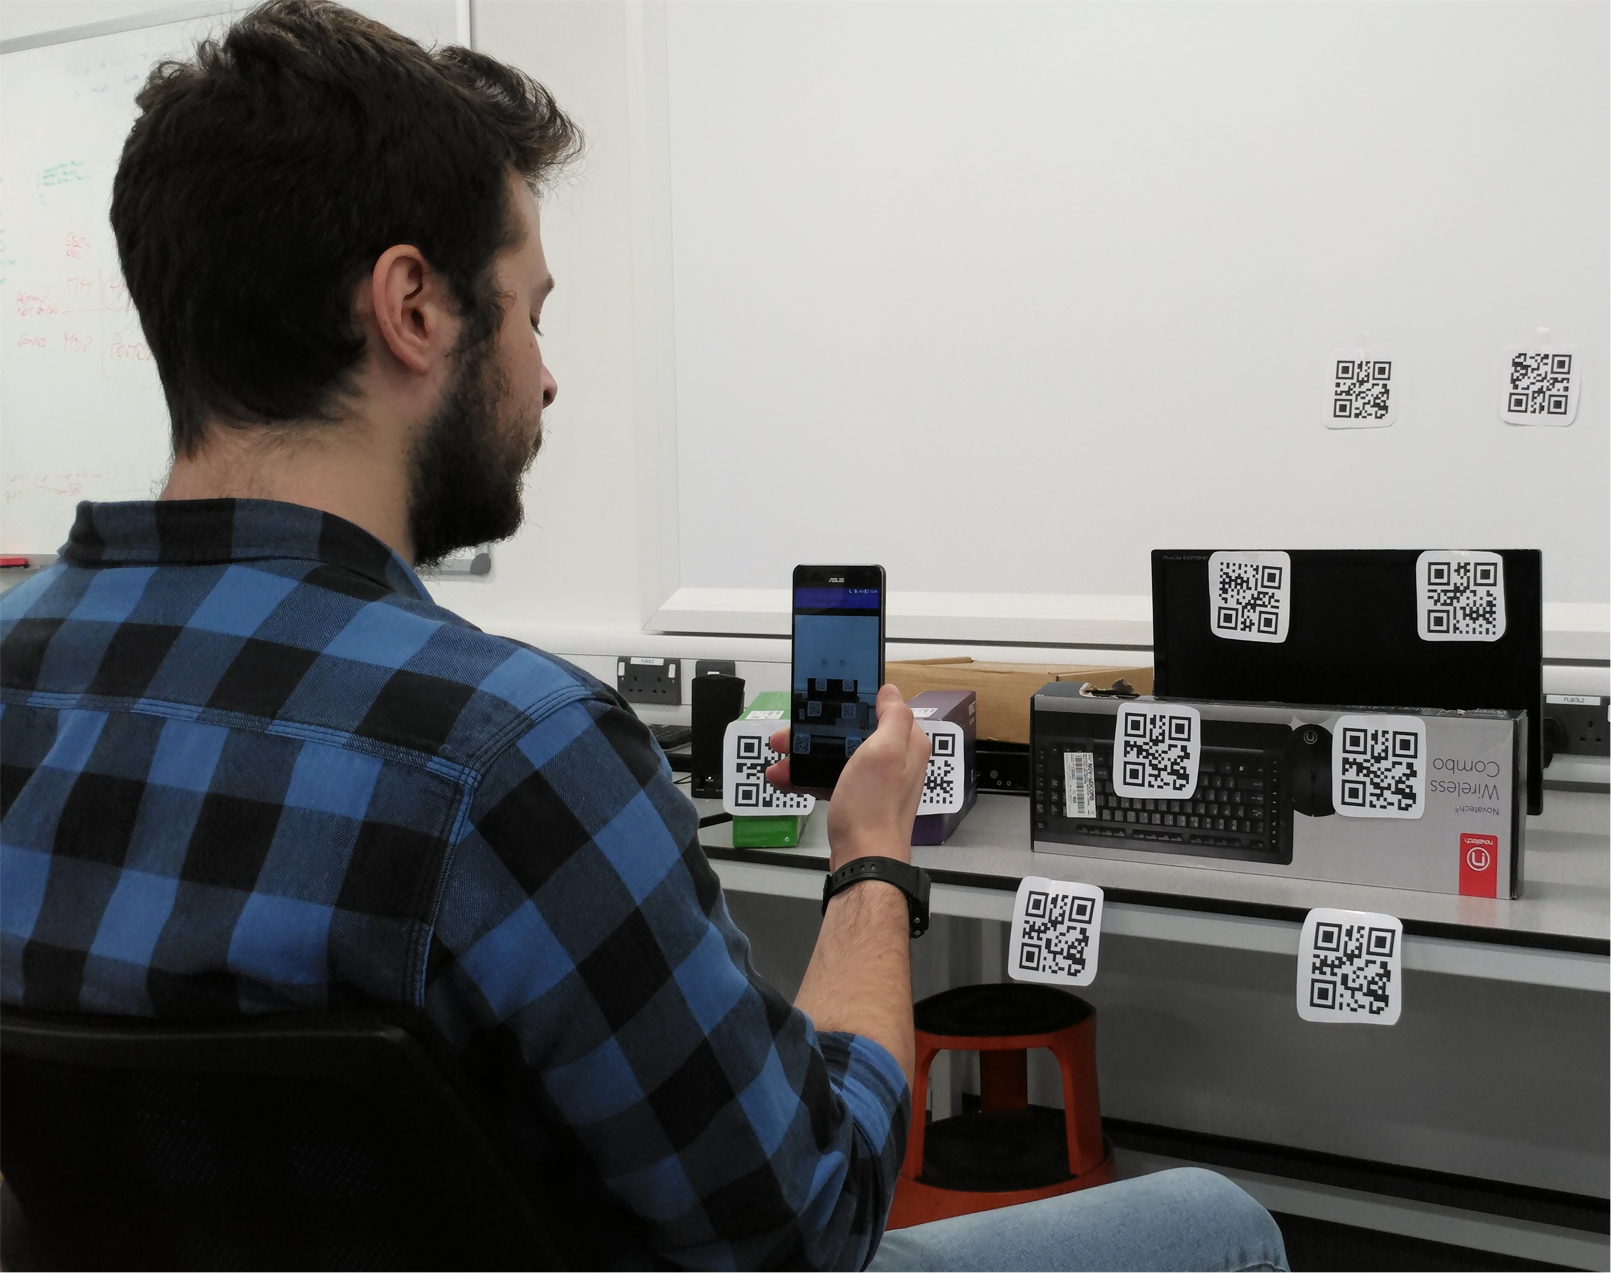
\includegraphics[width=0.38\textwidth]{../figures/system_use.png}
  \caption{The system in use during an experiment. }\label{fig:system-use}
\end{figure}

The goal of our active search system is to understand the user's surroundings and determine what the next best course of action is to reach the target object based on what is currently within view and what has been observed in the past. To this end, we implemented a smartphone guidance system based on a Markov Decision Process (MDP)~\cite{bellman1957markovian} that generates, in real-time, a series of instructions for the user to point to the target, depending on a previously-learned spatial distribution of known objects and on the camera's current view.  
%
This work includes three main contributions:

\begin{itemize}
  \item an MDP-based human controller that can guide a user in a visual search task;
  \item a data-based transition model for the MDP which includes spatial relations between known objects;
  \item a set of user experiments that prove the effectiveness of our active search implementation.
\end{itemize}

%is the design of a guidance system and MDP (the control-block, $K$, pictured in Figure~\ref{fig:control-loop}) that can drive a user to point a mobile device's camera towards a given point in space in and find a target object. We also present and discuss preliminary experimental results to show how effective the system is at finding a target. This guidance system will be implemented into the ActiVis project upon successful tests. 

Section~\ref{sec:previous-work} discusses other relevant work done in this field, followed by a general explanation of the active vision system for human guidance in Section~\ref{sec:system-design}, and a detailed explanation of the human-control module in Section~\ref{sec:controller-design}. The experimental results are presented in Section~\ref{sec:experiments}, after which we conclude the paper and discuss future work in Section~\ref{sec:conclusion}. 

\section{\uppercase{Previous Work}}\label{sec:previous-work}

\noindent Assistive vision and guidance for people living with vision impairments is a growing research area. In recent years, the increase in mobile processing power and computer vision improvements have led to research in the use of smartphone cameras to augment or enhance a user's vision and help them find objects or other points of interest. Earlier attempts at the problem involved placing special markers or barcodes around an environment, which the user then scans with a smartphone or similar mobile device~\cite{gude2013blind,iannizzotto2005badge3d,manduchi2012mobile}. This device then uses some feedback mode, e.g.\ Braille or sound, to guide the user towards the target. %The major drawbacks to this approach is the significant upfront effort required to augment entire areas with markers to a point where the system will be useful to a VI user. Furthermore, these passive systems rely on the user scanning the marker in the first place; something that can be made more complicated with markers degrading over time, changing ambient lighting, different viewing angles and marker occlusion. 

Another approach is to discard tags completely and rely on computer vision to perform the object detection, something that has become more practical with recent improvements to feature detectors and deep networks~\cite{huang2017speed,redmon2016you}. SIFT and SURF-based object detectors have also been used to detect known objects, when they are in the camera's view, and to guide the user to them using sonified instructions~\cite{schauerte2012assistive}. These type of systems is more flexible than the tag-based ones, but it has the same drawback of being {\em passive}, in the sense that it relies on having the object within the camera's view in the first place. Also, no clear performance metrics are reported in the previous paper. The VizWiz system~\cite{bigham2010vizwiz} offloads the object recognition tasks to an Amazon Mechanical Turk worker who then provides feedback on where the object of interest is located relative to the user. The VizWiz has the advantage of being fairly robust and is able to classify a great deal of objects with little effort from the user and can provide natural, human-generated and curated directions. However, this approach does not enhance user independence, since a person with vision impairments is now beholden to an online worker instead of a relative, friend or bystander. Furthermore, a good internet connection is required on the device, possibly limiting its use in some poor-reception areas.

Previous researchers have implemented active search and perception strategies in robots and image classifiers~\cite{Bajcsy2017} in an attempt to optimise their classification and planning tasks, for example by exploiting the structured nature of human environments and object placements. 
%
Two research teams have recently implemented an active object search strategy into their image classifiers~\cite{caicedo2015active,gonzalez2015active}. Their approaches use different methods, but conceptually similar models to generate windows of interest for visual classification. The size and locations of the windows within the image are generated using the spatial relationship between objects, taken from the SUNCG and PASCAL datasets~\cite{song2016ssc,Everingham10}, and are iteratively changed based on the output from the respective models. The advantage of their approaches is that fewer windows are generated and submitted to the classifier, resulting in lower object classification times while still keeping state-of-the-art results for accuracy. 

Similar strategies have been incorporated on robotic platforms to improve autonomous object search, manipulation and localisation tasks. For example, some researchers have developed a planning algorithm for a robotic manipulator that performs an optimal object search in a cluttered environment~\cite{dogar2014object}. Another team implemented an MDP generating an optimal object search strategy in a room over a belief state of object positions and configurations~\cite{aydemir2011search}. However, the authors trained their MDP using a custom object-placement and configuration scenario, so their results are sensitive to changes within this distribution. 

In summary, much research has been conducted on recognition of and guidance towards target objects, including active vision solutions for image classifiers and robotic systems. However, to our knowledge, no previous work has been done on {\em active} object search and guidance for humans, which would especially benefit people with vision impairments. In this paper, we implement such an active vision system with a human in the loop
% ~\cite{bellotto2013,lock2017portable}
that guides the user towards an out-of-view target object. Our system exploits prior knowledge of the objects spatial distribution within an indoor environment, learned from a dataset of real-world images, and the history of past object observations made during the search.
%With this, we hope to make the searching process less random and move towards a more natural and efficient object searching process to the benefit of the VI\@.  

\section{\uppercase{Active Vision System}}\label{sec:system-design}

\noindent The work presented in this paper is a fundamental step towards a more general project's goal to develop a stand-alone system that can guide a user living with vision impairments to their destination with minimal user input or intervention. A complete system diagram is given is Figure~\ref{fig:control-loop}. This closed-loop system is conceptually similar to other classical control problems, where the difference between desired and actual state of a process is used to generate a control signal that changes the process itself.

\begin{figure}
  \centering
  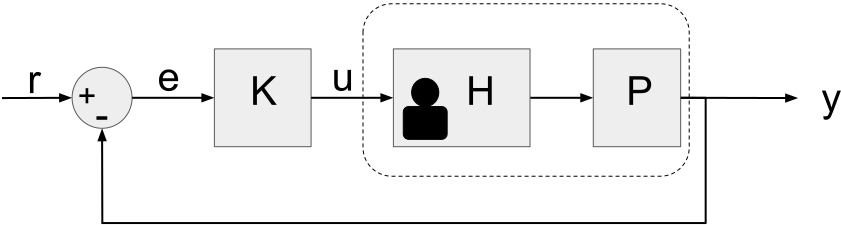
\includegraphics[width=0.45\textwidth]{../figures/control_loop.png}
  \caption{System control loop: $r$ is the reference object, $e$ the error signal, $u$ and $u^*$ the original and interpreted control signals and $y$ is the current object observation. $K$, $H$ and $P$ are the control, human and sensor blocks respectively. }\label{fig:control-loop}
\end{figure}

In this case, the reference signal, $r$, is the object the user wishes to capture with the smartphone's camera. The goal of the control block, $K$, is to generate human interpretable instructions, $u$, to guide the user towards the target object. The process to be controlled involves a human, $H$, who interprets the instruction and executes a physical action, $u^*$, to actually manipulate the smartphone's camera, $P$. A new observation, $y$, with the camera is then fed back to the loop and the error signal, $e$, is updated accordingly.  

Here we focus in particular on the implementation of the control module $K$. Two important points are considered in the design of the controller. Firstly, $K$ must be scenario-agnostic, meaning that objects could be placed in different places with unknown a priori. Secondly, the controller must be robust enough to handle incorrect interpretations by the human of the instructions $u$. Since each person interprets audio signals differently (modelled by the transformation block $H$), this is an important consideration. For example, one person might interpret and execute an `UP' instruction correctly (i.e. $u\approx u^*$), while another might interpret it correctly, but execute an incorrect action. This risk can be mitigated by the use of clear and simple instructions that helps $u$ track $u^*$ as closely as possible. The implementation of this controller is discussed in detail next. 

\section{\uppercase{Human-control Module}}\label{sec:controller-design}

\noindent Our active search system guides the user by generating a set of waypoints that need to be observed by the camera, tracing a path that will eventually lead to the target object. Note that the actual location of the latter is {\em unknown}, meaning that the system will guide the user towards the most likely location where the object might be found, based on its internal knowledge of spatial relations between objects (e.g.\ a computer monitor is more likely to be above than below a desk). This path is generated one waypoint at a time and is updated with every new object observation captured by the camera, or after a re-orientation of the latter beyond a certain angle. We tackle the problem using an MDP, the design and implementation of which are discussed in the following sub-sections. %For this initial design, the system only works in the pan and tilt dimension and the depth dimension will be added after successful testing of this version of the guidance system.
 %The guidance system is built into an Android app and uses Android's ARCore API to track the device's pose. 
%\subsection{Environment Model}\label{sec:env-design}

%\noindent We model this problem on the familiar grid-world problem, where an agent is tasked move to a terminal square from an origin square given some constraints. However, instead of the traditional, linear grid-world problem, we use the grid in a radial coordinate system which surrounds the user and each grid square represent a pan/tilt angle coordinate. See Figure~\ref{fig:environment} for an example grid. Since we do not consider the depth dimension yet, each grid square is equidistant from the user and agent. The agent translates between the squares as the user points the camera in different directions.

%\begin{figure}  
  %\centering
  %\tikzset{cross/.style={cross out, draw=black, minimum size=2*(#1-\pgflinewidth), inner sep=0pt, outer sep=0pt},cross/.default={1pt}}
\begin{tikzpicture}%[background rectangle/.style={fill=yellow!20}, show background rectangle]

  \def\thet{135}
  \def\ph{45}
  \def\l{2.2cm}
  \coordinate (O) at (0,0);
  \coordinate (U) at (3.5,-0.5);

  \node[below] (user) at ($(U)+(0,-0.4)$) {User};
  \draw[fill=black] (U) circle (0.3cm);

  \node[above] (gridlabel) at (2.3, 7.2) {Grid-world};

  % Draw the grid world outlines
  \coordinate (s0) at (0,0);
  \coordinate (s1) at (5,1);
  \coordinate (s2) at (5,6);
  \coordinate (s3) at (0,5);
  \draw[name path=bot_curve] (s0) to[out=90, in=140] (s1);
  \draw (s1) -- (s2);
  \draw[name path=top_curve] (s2) to[out=140, in=90] (s3);
  \draw (s3) -- (s0);% node[above right] {(0, 0)};

  %Draw horizontal grid lines 
  \draw[dashed] ($(s0)+(0,1)$) to[out=90, in=140] ($(s1)+(0,1)$);
  \draw[dashed] ($(s0)+(0,2)$) to[out=90, in=140] ($(s1)+(0,2)$);
  \draw[dashed] ($(s0)+(0,3)$) to[out=90, in=140] ($(s1)+(0,3)$);
  \draw[dashed] ($(s0)+(0,4)$) to[out=90, in=140] ($(s1)+(0,4)$);
  \draw[dashed] ($(s0)+(0,5)$) to[out=90, in=140] ($(s1)+(0,5)$);

  % Draw vertical grid lines
  \coordinate (v1) at ($(s0)!0.166!(s1)$);
  \coordinate (v2) at ($(s0)!0.33!(s1)$);
  \coordinate (v3) at ($(s0)!0.5!(s1)$);
  \coordinate (v4) at ($(s0)!0.66!(s1)$);
  \coordinate (v5) at ($(s0)!0.83!(s1)$);

  \draw[draw=none,name path=vert1] (v1) -- ($(v1)+(0,7)$);
  \draw[draw=none,name path=vert2] (v2) -- ($(v2)+(0,7)$);
  \draw[draw=none,name path=vert3] (v3) -- ($(v3)+(0,7)$);
  \draw[draw=none,name path=vert4] (v4) -- ($(v4)+(0,7)$);
  \draw[draw=none,name path=vert5] (v5) -- ($(v5)+(0,7)$);
  \coordinate[name intersections={of=bot_curve and vert1,by={int11}}];
  \coordinate[name intersections={of=top_curve and vert1,by={int12}}];
  \coordinate[name intersections={of=bot_curve and vert2,by={int21}}];
  \coordinate[name intersections={of=top_curve and vert2,by={int22}}];
  \coordinate[name intersections={of=bot_curve and vert3,by={int31}}];
  \coordinate[name intersections={of=top_curve and vert3,by={int32}}];
  \coordinate[name intersections={of=bot_curve and vert4,by={int41}}];
  \coordinate[name intersections={of=top_curve and vert4,by={int42}}];
  \coordinate[name intersections={of=bot_curve and vert5,by={int51}}];
  \coordinate[name intersections={of=top_curve and vert5,by={int52}}];
  \draw[dashed] (int11) -- (int12);
  \draw[dashed] (int21) -- (int22);
  \draw[dashed] (int31) -- (int32);
  \draw[dashed] (int41) -- (int42);
  \draw[dashed] (int51) -- (int52);
  
  % Draw user node and viewing angles
  \coordinate (c) at ($(U)+({\l*cos(\thet)}, {\l*sin(\thet)})$);
  \coordinate (cpan) at ($(c)+({-tan(\ph)*cos(\ph)}, {-tan(\ph)*sin(\ph)})$);
  \coordinate (ctilt) at ($(c)+({tan(\ph)*sin(\ph)}, {tan(\ph)*cos(\ph)})$);

  \draw[-Latex,] (U) -- coordinate (carc) (c) node[below] {C};
  \draw[dashed,-Latex] (U) -- coordinate (cpanarc) (cpan);
  \draw[dashed,-Latex] (U) -- coordinate (ctiltarc) (ctilt);

  \draw[-Latex] (carc) to[out=190, in=80] (cpanarc) node[right, yshift=0.13cm] {$\phi$};
  \draw[-Latex] (carc) to[out=80, in=190] (ctiltarc) node[below left] {$\theta$} ;

  % Add objects
  \coordinate (obj1) at ($(v1)!0.5!(v2) + (0,1.8)$);
  \coordinate (obj2) at ($(v3)!0.5!(v4) + (0,3.7)$);
  \coordinate (obj3) at ($(v2)!0.5!(v3) + (0,4.8)$);

  \draw (obj1) node[cross=3pt,rotate=12] {};
  \draw (obj2) node[cross=3pt,rotate=-3] {};
  \draw (obj3) node[cross=3pt,rotate=4] {};

  \node[left] (objectlabel) at (-0.4,2) {Objects};

  \draw[->] (objectlabel) -- ($(obj1)+(-0.1,0)$);
  \draw[->] (objectlabel) -- ($(obj2)+(-0.1,-0.1)$);
  \draw[->] (objectlabel) -- ($(obj3)+(-0.1,-0.1)$);

\end{tikzpicture}

%\caption{A diagram of the radial grid-world used in the MDP is modelled with. }\label{fig:environment}
%\end{figure}

%MDPs are well-suited to solving this class of problem, i.e.\ to find the optimal route from the origin square to the terminal square, so modelling our problem as a grid-world allows us to design our guidance system and MDP model with existing and well-understood models and techniques. Each square of the grid represents a combination of the agent's pan-tilt-observation, or state, which is discussed in more detail in Sec.~\ref{sec:states}. The terminal square is the square whose state contains the target object, or observation. The grid size can be adjusted to control the model's resolution: smaller squares will increase accuracy, but at the cost of performance, both during use (more squares need to be traversed) and training (much larger state space). For the initial system design, we set the grid resolution to \SI{30}{\degree}.

\subsection{MDP for Human Control}

\noindent An MDP produces a policy of optimal actions for an agent to take in any given pre-defined state. In this case, the agent is defined as the guidance system and the policy is used to generate the next waypoint on the search path towards the target object. We assume fully observable states and known state transitions probabilities. The MDP is represented by the 5-tuple

\begin{equation}
  (\mathbf{S}, \mathbf{A}, \mathbf{T}, \mathbf{R}, \gamma),
\end{equation}
where $\mathbf{S}$ is a set of possible agent' states, $\mathbf{A}$ is a set of possible actions the agent can take in any given state, $\mathbf{T}$ is a set of state transition probabilities from state $s$ to state $s'$, with ${s,s'~\in~\mathbf{S}}$, and $\mathbf{R}$ is the reward the agent receives for reaching state $s'$ after executing action $a \in \mathbf{A}$ in state $s$. The scalar $\gamma$ is a discount factor which prioritises immediate over long-term rewards and affects the model's convergence rate. Each of these elements are defined and discussed next.

\subsubsection{States}\label{sec:states}

\noindent The state is a combination of parameters that defines the agent's world and decision process. Our state vector is defined as

\begin{equation}
  s = \langle o, n, v \rangle, 
\end{equation}
where $o$ is the current object in viewed by the camera, $n$ is the number of steps taken since the search started, and $v$ is a binary variable that keeps track of whether a waypoint for the current state was already generated during the current object search. 

\subsubsection{Actions}

The policy produced by an MDP define the action the agent will take when it finds itself in any given state. In this case, the action is the direction of the next waypoint relatively to the current device's pose. The possible actions are given by

\begin{equation}
  \mathbf{A} = \{UP, DOWN, LEFT, RIGHT\}.
\end{equation}
%These actions were chosen to conform to the grid implementation and increase the tracking performance of $u^*$ w.r.t\@ $u$. 

To illustrate an example of actions sequence, let us consider the scene in Figure~\ref{fig:route-example}, which contains a number of simple, distinct objects (red boxes). The MDP guides the user in pointing the camera to the target object (the mug at the bottom-left of the figure). It does this by inferring the current state, which depends on the object currently observed by the camera, and generating an action, or instruction, that leads the user to the target object.
%The states are sampled and the actions are generated in discretised steps as the user moves the camera's view in the instructed direction. %This discrete behaviour is similar to a waypoint navigation approach where the user goes from one waypoint to the next, until the user points the camera to target object. 
An action is considered completed, and therefore a new state reached, when the camera has rotated more than a predefined angle or a new object is detected.

\begin{figure}
  \centering
  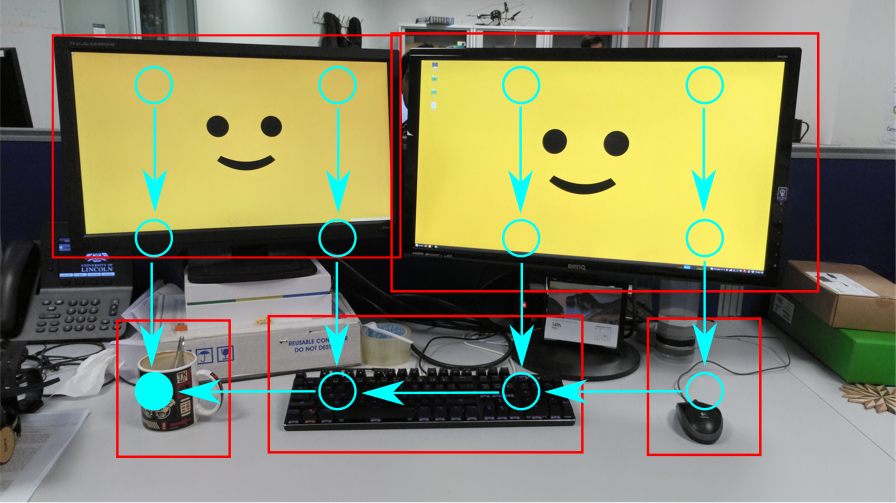
\includegraphics[width=0.5\textwidth]{../figures/office_desk_example.png}
  \caption{An example action policies generated by the MDP to guide the user in pointing the camera from a random starting object (e.g. monitor) to a target object (e.g. mug). }\label{fig:route-example}
\end{figure}

\subsubsection{State Transition Probabilities}

\noindent The state transition $\mathbf{T}$ defines the probability of the agent switching from state $s$ to state $s'$ due to action $a$, i.e.\ the probability of observing object $o'$ after object $o$ due to a pan/tilt rotation of the camera. Therefore, $\mathbf{T}$ represents the spatial relationships between the different objects in our environment model. 
% Formally, the transition function is defined by
% 
% \begin{equation}
%   t=\langle{}s, a, s'\rangle, t\in{}\mathbf{T}.
% \end{equation}
These spatial relationships are learned from a dataset during an initial training process, which is discussed more in detail in Section~\ref{sec:training}.

\subsubsection{Reward Function}

\noindent The reward $\mathbf{R}$ is the immediate reward that the agent receives after transitioning from state $s$ to state $s'$.
% and is given by 
% 
% \begin{equation}
%   R\in r(s, s').
% \end{equation} 
% 
The goal of the agent is to maximise its cumulative reward and it is very important to fine-tune $\mathbf{R}$ correctly in order to produce an effective action policy. In order to encourage the agent to find the target object as fast as possible, a relatively large positive reward should be assigned for successfully reaching the goal state, and a negative one in any other case. These parameters must be finely balanced to ensure effective object search behaviour.

%The reward function is a very important parameter for training the agent to produce the most effective policy. We define a constant negative reward for every step the agent takes, and increase this negative reward if the agent exceeds the 12-step limit we defined in the model, as well as if it regenerates a waypoint in a previously searched location. The values we used were empirically chosen and are given in Table~\ref{tab:rewards}.

%The goal of the agent is to maximise its cumulative reward over time and these numbers are chosen such that they actively motivate the agent to reach the target, while hastening the process by slightly punishing it for each step it takes and increasing the punishment every time it re-explores a state and the longer it takes to reach the target. 

\subsection{MDP Implementation}

This section describe the actual implementation details of the MDP for active object search, including initial training and software deployment on our smartphone device.

\subsubsection{Training} \label{sec:training}

\noindent A policy that defines the optimal action for an agent to take for any given state is generated through a training process that involves letting the agent explore the entire state-space and iteratively improve its decision function, i.e.\ policy, in order to reach the target state in a way that maximises its cumulative reward. This method, called Q-learning~\cite{Watkins1992}, does not require a model of the agent's environment during training, allowing the policy to be used in many different scenarios.

Currently there are 7 objects encoded into the system, plus a `nothing' instance where nothing of note is observed. Our initial implementation considers a simple office desk scenario containing the following objects:

\begin{equation}
  \begin{aligned}
    o\in \mathbf{O} = \{monitor, mouse, keyboard, window,\\mug, stationery, desk, nothing\}.
  \end{aligned}
\end{equation}

The spatial relationships between the objects in $\mathbf{O}$ are extracted from the OpenImage dataset~\cite{openimages}, which consists of 1.74M images containing 14.6M manually drawn and labelled bounding boxes around objects (see Figure~\ref{fig:openimage-example} for an example). The dataset is primarily aimed toward object recognition researchers to benchmark their models. In our case though, the bounding boxes and object labels are used to extract the spatial relationships between the different objects in $\mathbf{O}$. Since the camera perspectives and absolute distances between the objects in the images are not given, we can only extract the relationships in the basic action terms specified in $\mathbf{A}$, e.g. we can only say that object 1 is above object 2, but not how far above. Our relatively simple action-space is therefore suitable for the dataset's lack of information. 

\begin{figure}
  \centering
  \begin{subfigure}
    \centering
    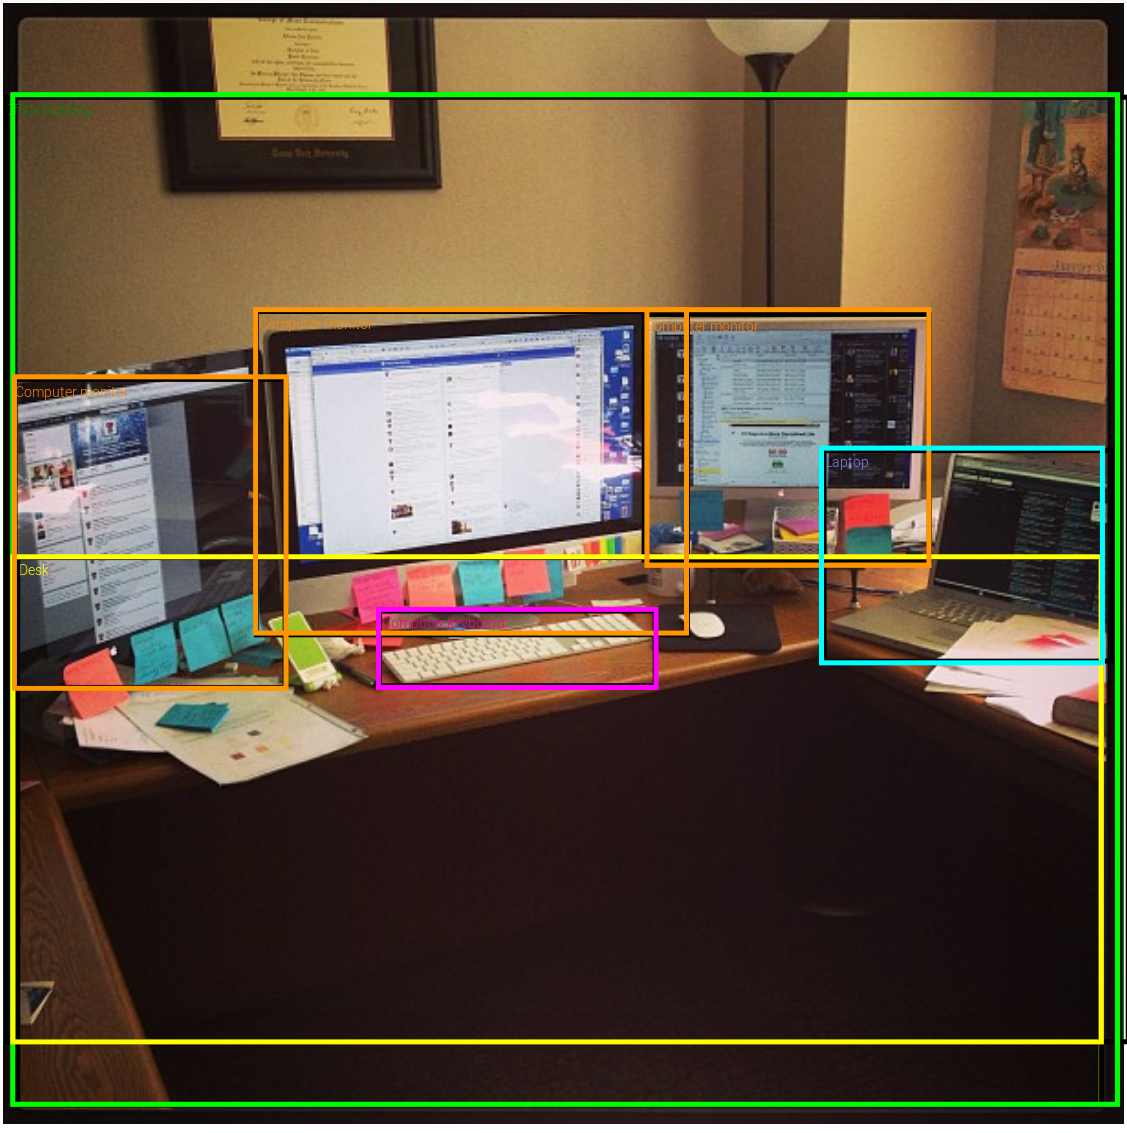
\includegraphics[width=0.4\textwidth]{../figures/desk_example.png}
  \end{subfigure}
  \begin{subfigure}
    \centering
    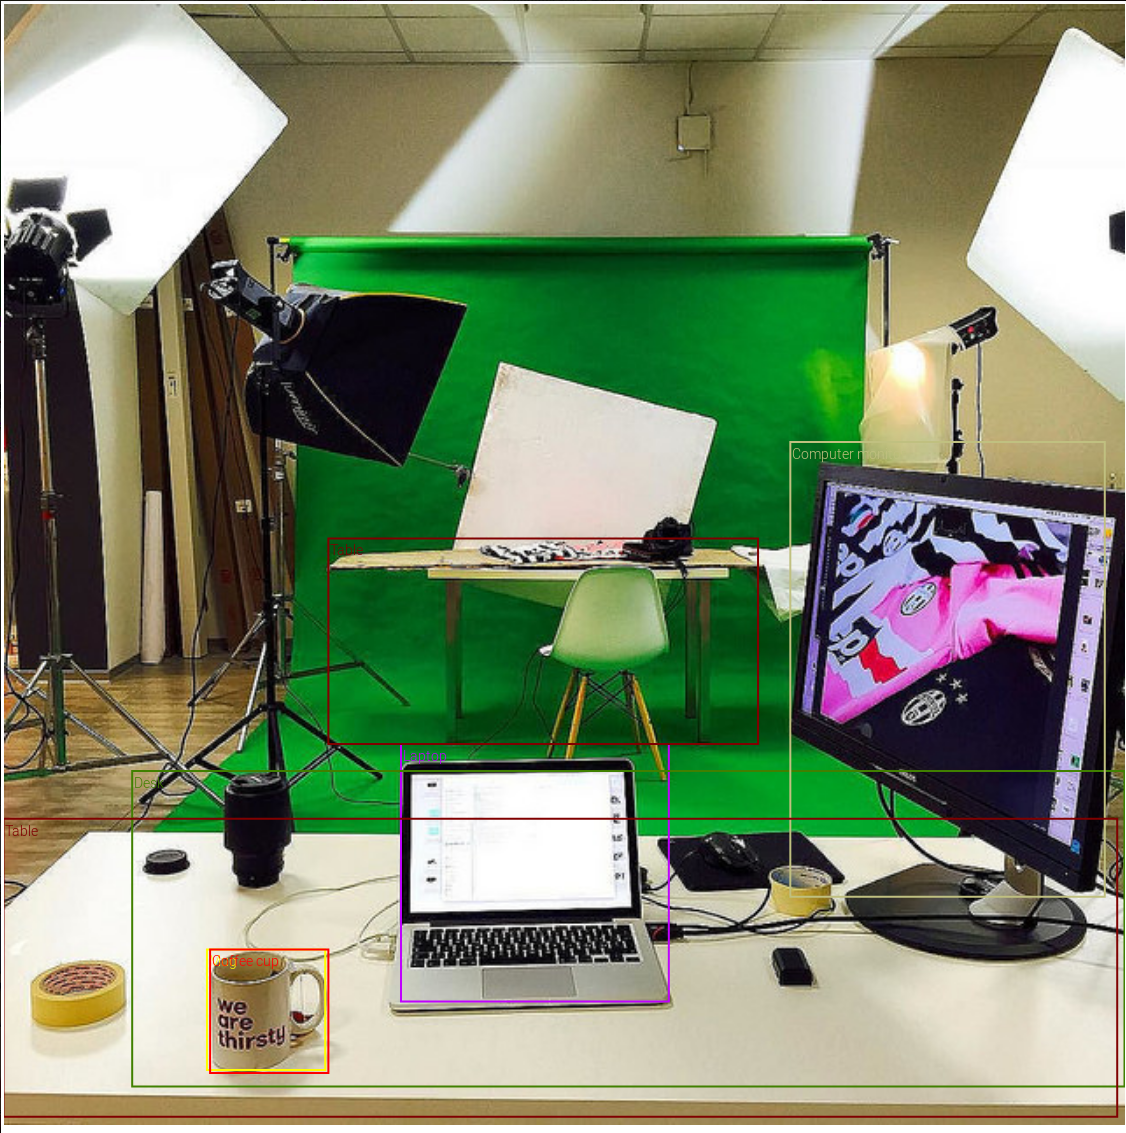
\includegraphics[width=0.4\textwidth]{../figures/mug_example.png}
  \end{subfigure}
  \caption{Examples of images from the OpenImage dataset containing objects from $\mathit{O}$~\cite{openimages}. }\label{fig:openimage-example}
\end{figure}

Figure~\ref{fig:obj-relationships} shows the spatial relationship between a subset of $\mathbf{O}$ (desk, keyboard and mouse). For example, when the agent is in state ${s=\langle o=mouse, n, v \rangle}$ and is searching for the object $o_{target} = keyboard$, there is a strong probability that the target object is on the mouse's $LEFT$. The MDP of course will consider all of the objects' spatial relationships when generating the optimal policy.

\begin{figure}
  \centering
  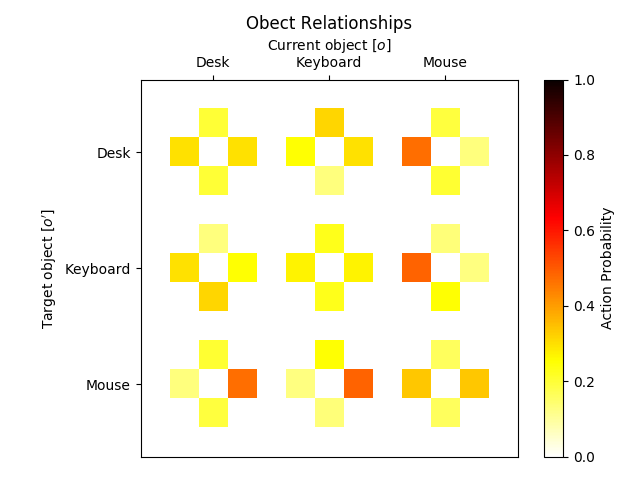
\includegraphics[width=0.5\textwidth]{../figures/object_relationships.png}
  \caption{Examples of the spatial relationships between the desk, keyboard and mouse objects. Each square corresponds to the probability of executing an action (top square for $UP$, left square for $LEFT$, etc.)}\label{fig:obj-relationships}
\end{figure}

The agent's target state is then any state where ${s = \langle o=o_{target}, n, v \rangle}$. This gives a total of 14 terminal states (7$\times$2) per policy, since the target object can be found at any point in the search or in a position that was previously explored by the user. Each target object has its own unique policy file.

The reward function was hand-crafted and the parameters were empirically selected. The function values can be found in Table~\ref{tab:rewards}. The reward punishes the agent for every step it takes without finding the target object. The reward becomes increasingly negatives as the agent progresses without finding the target~($n > n_{\max}$) or when it generates the same waypoint more than once~($v = true$) during the same search. Conversely, it gives a significant positive reward when the target object is found. 

\begin{table}
  \centering
  \caption{The reward functions for the MDP.\ }\label{tab:rewards}
  \begin{tabular}{cc}
    \toprule
    $r(o = o_{target})$ & 10000 \\ \midrule
    $r(v = true)$  & -10 \\ \midrule
    $r(n > n_{\max})$ & -10 \\ \midrule
    otherwise $r(\cdot)$ & -1  \\ \midrule
    \bottomrule
  \end{tabular}
\end{table}

We force the MDP to generate a maximum of 11 (inclusive) steps to the target, with 11 being the longest possible route on the action grid (more details about the grid are in Section~\ref{sec:system-implementation}). A search could take longer than 11 steps, but the MDP considers that the maximum, which is convenient for keeping a manageable state-space and a simple reward function. The MDP therefore has a total of 154 reachable states ($s_{total}=11\times7\times2$).

The lack of absolute spatial information in the OpenImage dataset generates ambiguities, which makes it hard for the model to converge to a single, optimal solution. We therefore opted to use the more conservative state-action-reward-state-action (SARSA) algorithm~\cite{rummery1994line}. SARSA is an on-policy algorithm that allows us to control the level of exploration vs.\ exploitation that makes it easier to find a solution, although this is not guaranteed to be optimal. 

The MDP is trained until it converges to the optimal policy, or for a total of approximately 17 million episodes. The parameter $\alpha$, which controls the exploration vs.\ exploitation behaviour during training, maximises the exploration when set to $1$ and the exploitation when $0$. We therefore set $\alpha$ to be a function of the training episodes, starting with a high exploration value and exponentially changing to exploitation as the training progresses: 

\begin{equation}
  \alpha = \exp\Big(\frac{-i}{10~s_{total}}\Big) - 0.001,
\end{equation}
where $i$ is the episode index.  $\gamma$ is set to 0.95 to prioritise long-term reward and guarantee convergence. 

Our MDP has a relatively small state-action space. Therefore, a solution can be found in a reasonable amount of time. However, it should be noted that adjusting the angle interval, or adding more actions or objects, can easily lead to an intractable size of the state-space. 

\subsubsection{Android Implementation}\label{sec:system-implementation}

We incorporated the trained MDP-based controller into an app (see Figure~\ref{fig:system-screenshot}) for an Asus ZenPhone AR smartphone, running Android 7.0, with Google's augmented reality toolkit (ARCore), which provides the necessary 3D pose of the device. No further software or hardware modifications were required. This app is responsible for generating the guidance instructions and tracking the camera sensor ($K$ and $P$ blocks in Figure~\ref{fig:control-loop}) throughout a search session. Tracking the camera's pose allows the app to infer the current state and choose the optimal action to take next. 

\begin{figure}
  \centering
  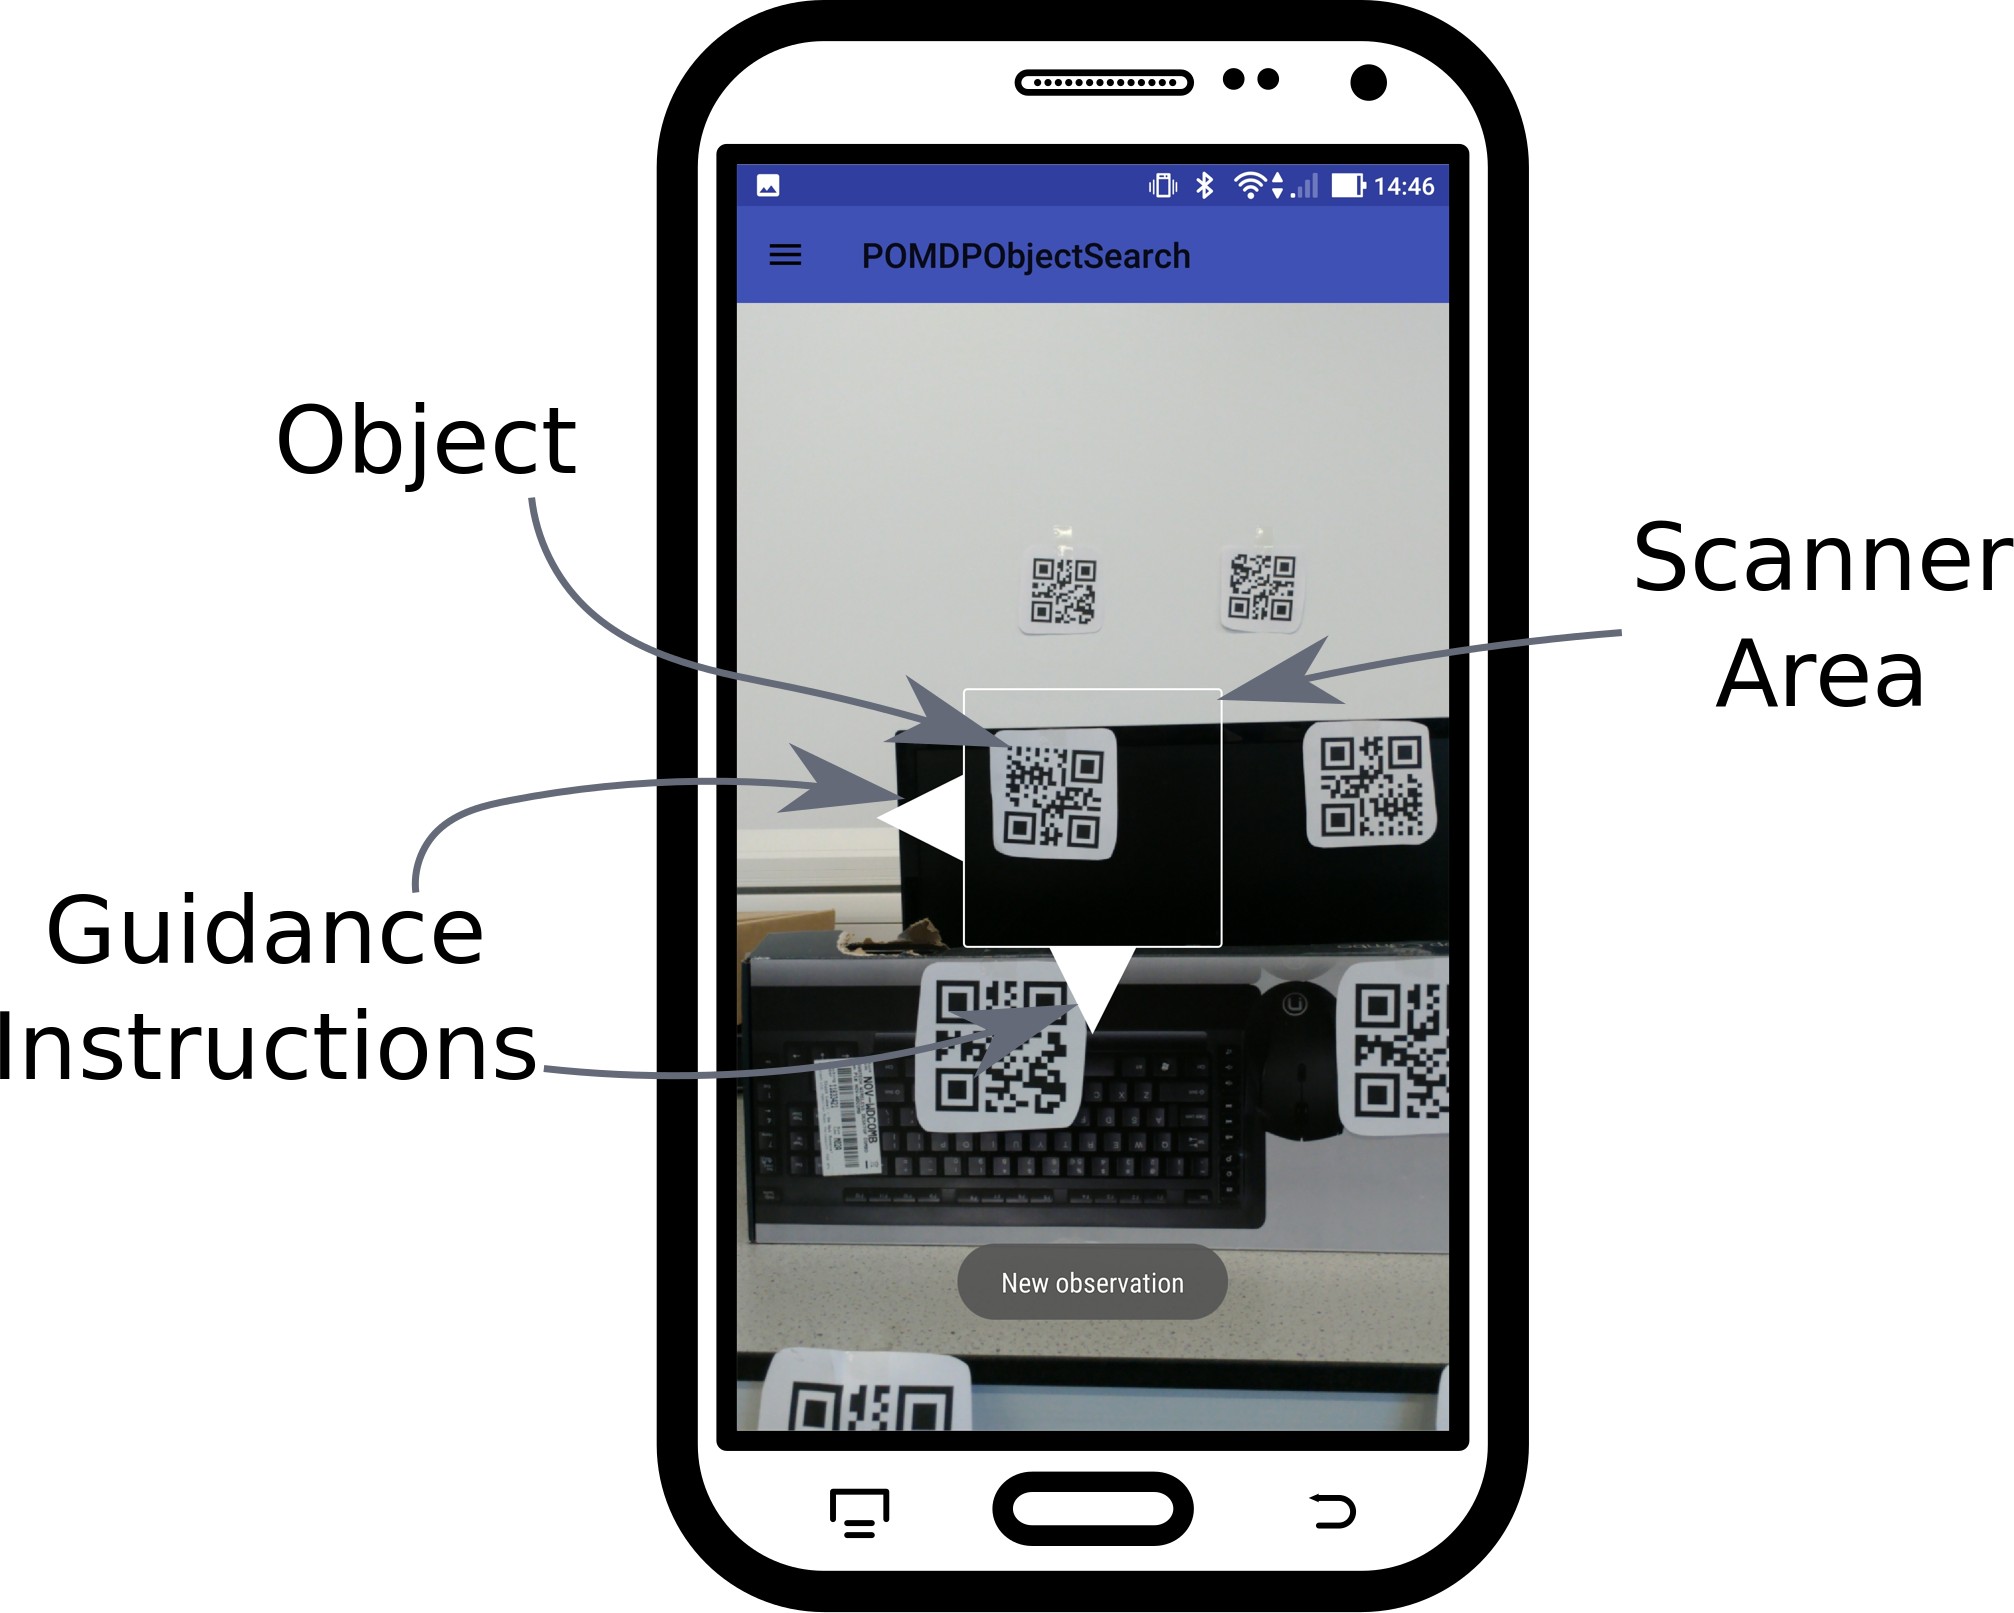
\includegraphics[width=0.35\textwidth]{../figures/system_screenshot2.png}
  \caption{A screenshot of the guidance interface showing an example of guidance instructions towards a waypoint and the QR-object scanner area.}\label{fig:system-screenshot}
\end{figure}

The app uses a 6$\times$6 discretised and wrapped radial grid to simplify the tracking and waypoint generation processes. The grid spans \SI{120}{\degree} in both the pan and tilt dimensions, giving a resolution of \SI{20}{\degree} per grid cell. A policy action is converted by the app into a new search waypoint centred on a cell of the radial grid, e.g.\ an `$UP$' action will generate a waypoint one grid cell above the camera's current orientation. Note that this cell is not part of the MDP's state and the radial grid is only used to discretise the pan-tilt movements of the camera and to guarantee a minimum angular variation between subsequent actions. The grid is generated at the app's start-up and remains constant throughout its lifetime. The app then uses the new waypoint's location to provide the user with guidance instructions. The policy actions, and waypoints by extension, are given relative to the current camera's pan-tilt orientation. The grid is wrapped, so if a waypoint's location exceeds the \SI{120}{\degree} limit, the waypoint is generated at the opposite side of the grid instead, limiting the search space to a \SI{120}{\degree}$\times$\SI{120}{\degree} area. 

The position of the waypoint is given to the user by a set of guidance instructions (the arrows seen on-screen in Figure~\ref{fig:system-screenshot}) in terms of the actions defined in $\textbf{A}$. This might seem like an unnecessary extra step, but this system is designed for user with vision impairments who are limited to audio instructions, which makes it necessary to split the instructions up into separate channels that can be communicated more simply. This requirement becomes clear when one considers the bandwidth limitations of a person's audio channel compared to the visual one. To clarify, the arrows were used for debugging and experimentation and they will be translated into audio signals once the audio interface is implemented.

By recording the previous positions and waypoint locations, the system can infer the state values for $n$ and $v$ described in Section~\ref{sec:states}. Furthermore, the camera provides the ID of the object currently within view, which is assigned to the state variable $o$. As explained in the next section, we did not use a real object detector in our experiments, but we simulated it with 7 different QR codes, one for each unique object, and a camera-based QR code scanner from Android's machine learning API (MLKit). 

The QR scanner requires raw image data. To avoid scanning multiple QR codes and speed up the image processing, we only used the central part of the camera's frame, which is $300\times300$ pixels. This choice also defines the precision required in pointing the camera towards the object (see also Figure~\ref{fig:system-screenshot}).

\section{\uppercase{Experiments}}\label{sec:experiments}

\noindent To test the effectiveness of our MDP and its policies, we designed a set of experiments that determined how effective the system is at directing a participant to point the device's camera towards a target object. This section discusses the experiments and their results. 

\subsection{Experiment Design}

\noindent For the experiment, the MDP policies were integrated into an Android application that uses the camera to provide observation data and track the pose and viewing direction. We avoided adding unnecessary variability and complexity to the experiment by providing visual waypoints on screen which the participants were allowed to use. A generic environment mimicking a typical office desk layout was set up as the experiment environment and contains 7 different objects (i.e.\ encoded QR codes), one of which could be selected for each experiment run. See Figure~\ref{fig:env-picture} for a picture of the environment. 

\begin{figure}
  \centering
  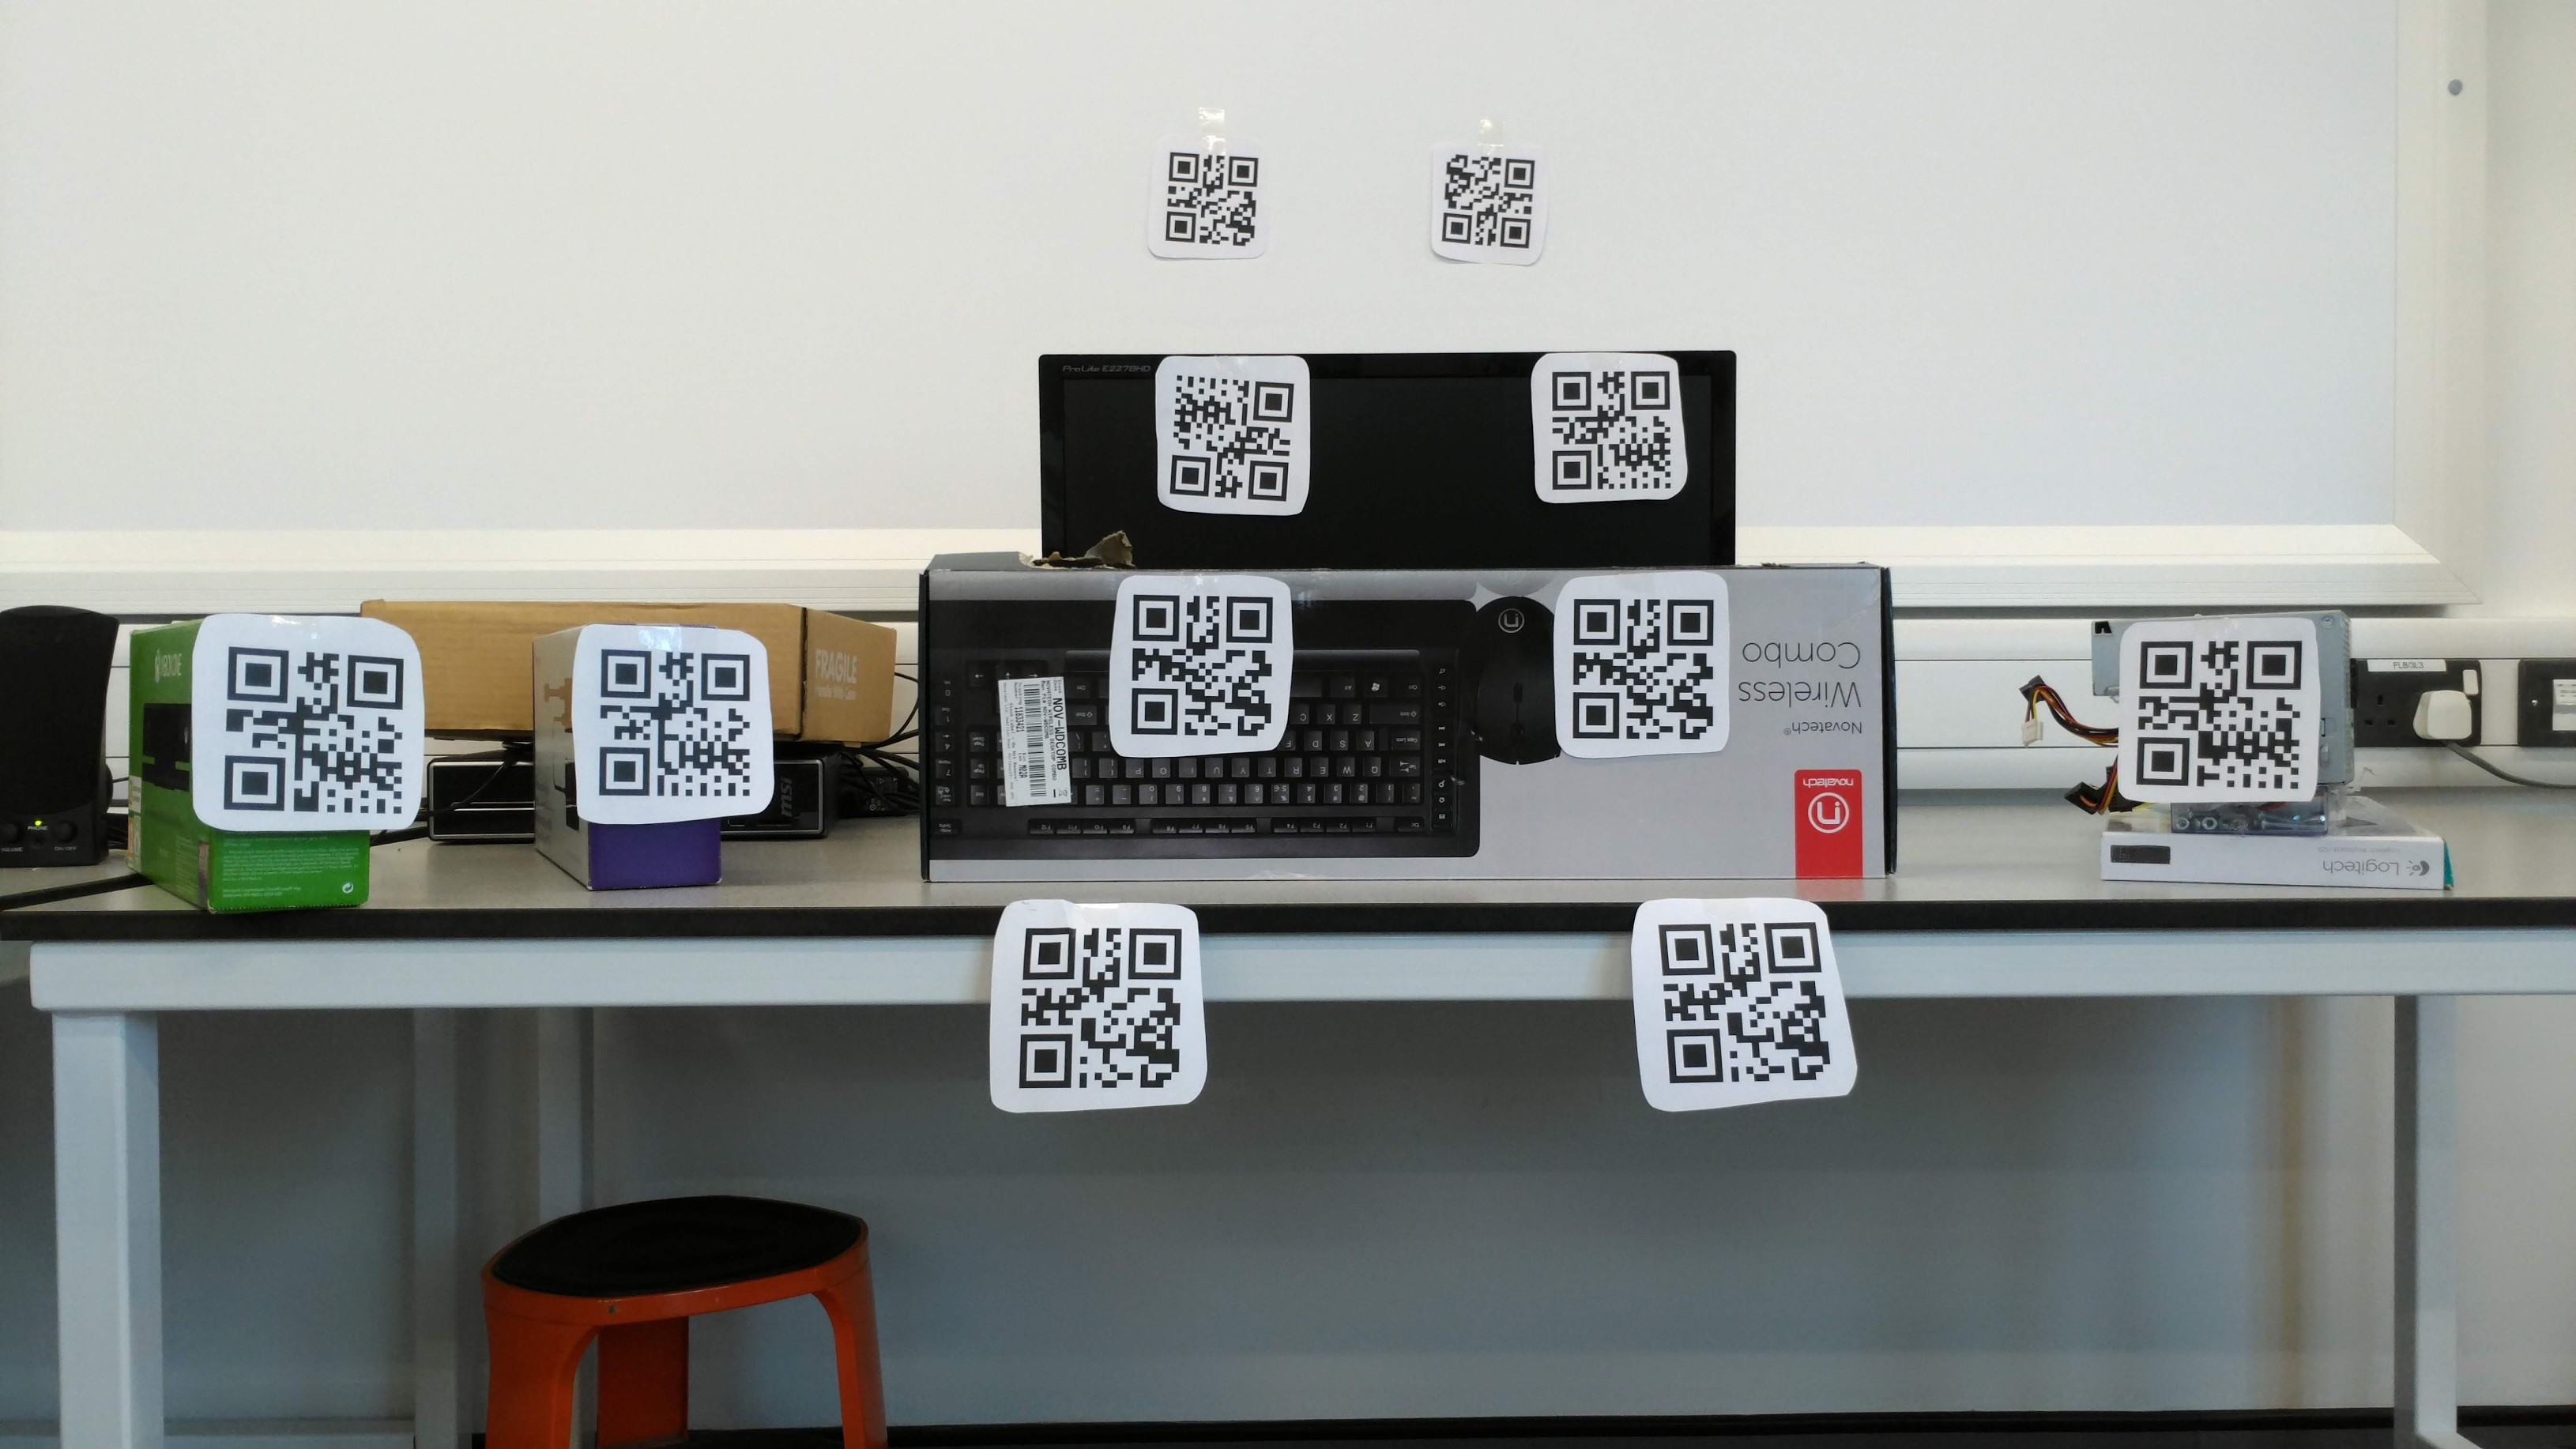
\includegraphics[width=0.45\textwidth]{../figures/test_env_picture.jpg}
  \caption{A picture of the environment used for the experiments. Each QR code represents an object.}\label{fig:env-picture}
\end{figure}

For each experiment, the participant was placed roughly \SI{1}{\meter} from the barcodes and was asked not to move from that spot during the experiment. The participant then pressed a button on the app that randomly selected a target object and was then guided towards that target by the app. Since the participants were allowed to use their vision, the targets were randomly selected and the participants were uninformed of what the target object was until it was found. This was done to avoid the participants learning the target objects' locations between each search run.

During in-house tests, we noted that the system sometimes makes guidance mistakes that lead the user towards an uncluttered edge of the search space, at which point the system had difficulty guiding the user back to the centre. To avoid this having an adverse impact and drawing out the experiments too long, we set a search step limit of 15, which means that the search was terminated when the number of waypoints exceeded 15. A search run therefore ended when the participant either successfully found the target object by pointing the phone camera to it and scanning the barcode, or exceeded the waypoint limit. After this, the participant then resets to the central position, selects a new target object and resumes the experiment.

The participants were left to repeat this process until we recorded 10 searches per object, giving us a total number of 70 recorded search samples per participant. We tested a total of 10 different participants (sex: 8 M, 2 F;\@ age: $\mu$ 31.2 years, $\sigma$ 8 years), most of whom were sourced from our laboratory. This gives our dataset a total of 700 search samples.

\subsection{Results}

\noindent We identified 3 different measures to evaluate the system's performance: target acquisition rate (TAR), number of steps to the target and the total time it took to find a target object. We present and discuss the results for each of these parameters in the next sections. The results for each individual participant is presented in Table~\ref{tab:results-full} and Table~\ref{tab:results-summary} gives the results across all of the participants. To provide a baseline measure for the ideal case, we ran a number of simulations in an environment mimicking the experiment setup with user that perfectly executes the policy, i.e.\ $u=u^*$. The TAR and steps to target results for the simulation are included in Table~\ref{tab:results-summary}.

\begin{table}
  \centering
  \caption{A table containing the results for the TAR, number of steps and time to target means and standard deviations for each participant. }\label{tab:results-full}
  \begin{tabular}{cccc}
    \toprule
    Participant & TAR [\%] & Num. Steps & Time [s] \\ \midrule
    %\multirow{2}{*}{Participant} & \multirow{2}{*}{TAR [\%]} & \multicolumn{2}{c|}{Num. Steps} & \multicolumn{2}{c}{Time [s]} \\ 
				 %&			     & $\mu$ & $\sigma$		       & $\mu$ & $\sigma$  \\ \midrule
    s1 & 94 & 7.2 $\pm$ 5.4 & 29 $\pm$ 22 \\ \midrule
    s2 & 79 & 6.7 $\pm$ 4.8 & 34 $\pm$ 5.1 \\ \midrule
    s3 & 91 & 6.3 $\pm$ 4.9 & 31 $\pm$ 21 \\ \midrule
    s4 & 79 & 6.7 $\pm$ 4.3 & 37 $\pm$ 5.6 \\ \midrule
    s5 & 76 & 7.2 $\pm$ 4.9 & 33 $\pm$ 14 \\ \midrule
    s6 & 60 & 8.2 $\pm$ 5.4 & 24 $\pm$ 10 \\ \midrule
    s7 & 86 & 8.5 $\pm$ 5.8 & 31 $\pm$ 16 \\ \midrule
    s8 & 88 & 5.1 $\pm$ 4.0 & 39 $\pm$ 21 \\ \midrule
    s9 & 98 & 7.2 $\pm$ 5.4 & 39 $\pm$ 18 \\ \midrule
    s10 & 67 & 6.6 $\pm$ 5.4 & 26 $\pm$ 12 \\ \midrule
    \bottomrule                    
  \end{tabular}                    
\end{table}                        
                                   
\begin{table}                      
  \centering                       
  \caption{The means and standard deviations for the entire participant population for the experiments and simulations.}\label{tab:results-summary}
  \begin{tabular}{ccc}
    \toprule
    \multirow{2}{*}{TAR [\%]} & Experiment & 82 $\pm$ 11  \\ 
			      & Simulation & 99.7 \\ \midrule
    \multirow{2}{*}{Num. Steps} & Experiment & 6.8 $\pm$ 5.1 \\ 
			        & Simulation & 5.4 \\ \midrule
    Time [s] & Experiment & 34 $\pm$ 23  \\ \midrule
    \bottomrule
  \end{tabular}
\end{table}

\subsubsection{Target Acquisition Rate}

\noindent The TAR is a measure of how successful the system was at directing a participant to the target object within the 15-step limit we set and is simply calculated as a proportion of the number completed searches vs.\ the total number of searches. Please note, however, that this plot is dependant on the step-limit we selected and should not be taken as an absolute measure of performance, but is rather presented to provide context to the other results we present. Figure~\ref{fig:tar-steps} shows the TAR as a function of the step-limit and it shows that there is a gradual increase in the TAR as the step limit increases, but tapers off as the step-limit increases.

\begin{figure}
  \centering
  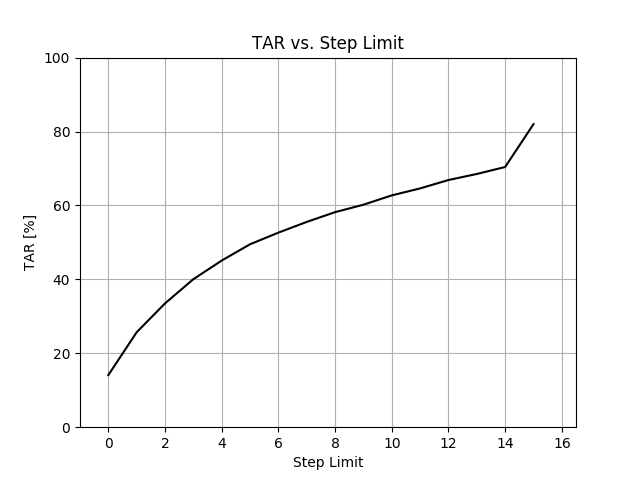
\includegraphics[width=0.5\textwidth]{../figures/cdf_tar_limit.png}
  \caption{The distribution of the TAR as a function of the step limit for a search. The `x' indicates the cases that exceeded the 15-step limit. }\label{fig:tar-steps}
\end{figure}

%\begin{figure}
  %\centering
  %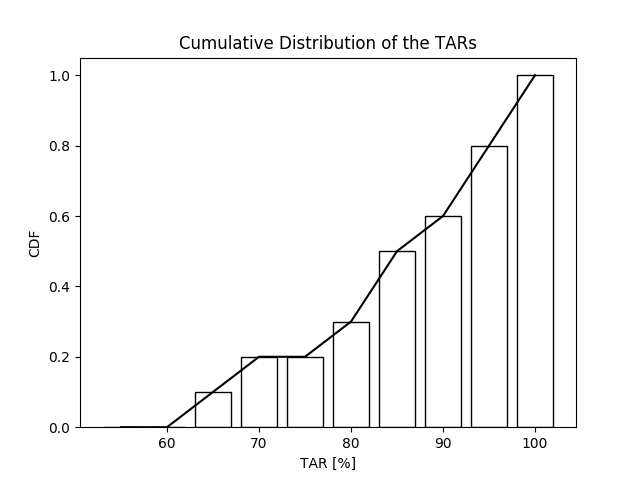
\includegraphics[width=0.5\textwidth]{figures/cdf_tar.png}
  %\caption{A plot giving the cumulative proportion of searches that successfully found the target object before reaching the 16-step limit. }\label{fig:complete-searches-subjects}
%\end{figure}

Table~\ref{tab:results-full} shows a fairly consistent spread for the TAR across the participants. The inter-participant spread ($\sigma=11\%$) is fairly significant, perhaps indicating that the user's search behaviour and strategy affects the target acquisition performance, but with an average TAR of $82\%$, it is clear that the system successfully finds the target object during the vast majority of searches. 

Figure~\ref{fig:tar-objects} shows the TAR for each object in $\mathbf{O}$. There are variations the TAR for the different objects, with the smaller objects typically being the hardest to find. However, the differences are not extreme and indicate that all the objects in $\mathbf{O}$ are roughly equally hard to find. This is also displayed in the simulation's TAR in Table~\ref{tab:results-summary}, which could not achieve 100\% because of the difficulty the agent had in finding the objects on the fringes of the environment. 

\begin{figure}
  \centering
  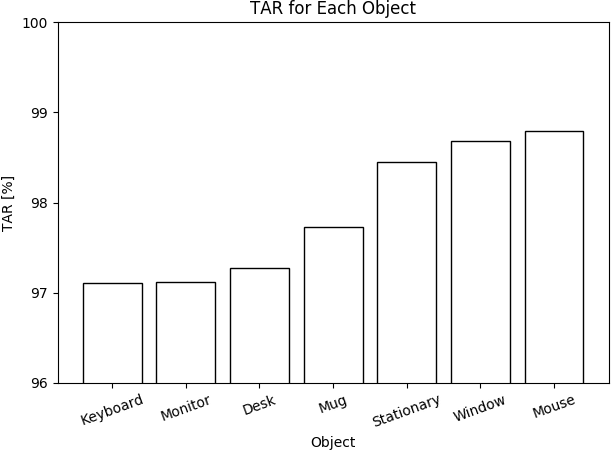
\includegraphics[width=0.45\textwidth]{../figures/tar_objects.png}
  \caption{The TAR for each of the objects within $\mathbf{O}$. }\label{fig:tar-objects}
\end{figure}

Failure cases were typically caused by the system entering a no-recovery state where the system directed a user into dead-space with no spatial information (e.g.\ a ceiling or wall section) and could not gather the information it required to intelligently guide the user. Subsequent system updates will have to consider implementing fall-back methods or automatic recovery modes that can detect entry of a no-recovery state (e.g.\ exceeding a set number of steps/time without making an observation) and guide the user back to the initial position and restart a search.

\subsubsection{Number of Steps to Target}

\noindent The number of steps to the target indicates the number of waypoints the system generated for the participant during the guidance process and is a major indication of system performance, where less waypoints means faster target acquisition and better performance. Figure~\ref{fig:nsteps-participants} shows the cumulative distribution of the number of steps to the target for all the participants. 

\begin{figure}
  \centering
  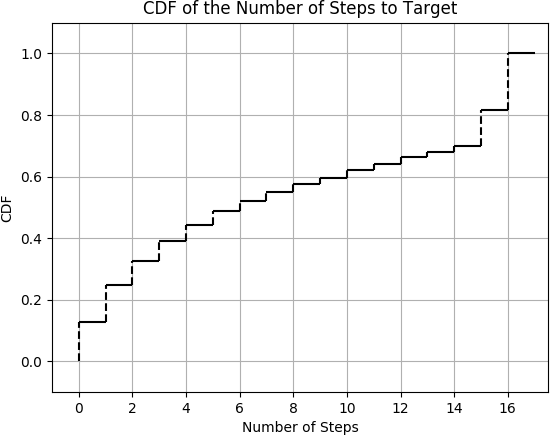
\includegraphics[width=0.5\textwidth]{../figures/cdf_total_steps.png}
  \caption{The cumulative distribution of the participants' number of steps taken to find a target object. }\label{fig:nsteps-participants}
\end{figure}

The number of waypoints each participant required is fairly evenly spread across all of the participants, with the majority of searches ending within 4 steps of initialisation or ending. The population mean and standard deviation is 6.8 and 5.1 waypoints respectively. This is a reasonable result, since most target objects were placed within approximately 4 grid squares away from the participants' initial looking directions. However, the relatively high standard deviation should be noted and can also be reduced by implementing the automatic recovery mode mentioned previously, and avoiding information-sparse areas.

%As expected, the number of steps the simulation required on average to find the target object is less than the participants did during the experiments. The full set of results for the simulation is given by a frequency mapping of the coincidences between the simulation and experimental data in Figure~\ref{fig:sim-vs-experiment}.

%\begin{figure}
  %\centering
  %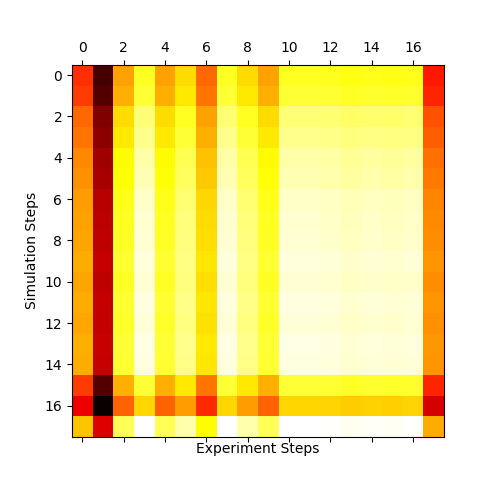
\includegraphics[width=0.5\textwidth]{figures/experiment_vs_simulation.png}
  %\caption{A summary of the experiment and simulation steps to target results. }\label{fig:sim-vs-experiment}
%\end{figure}

% It is interesting to note that participants $s6$ and $s10$ also found their targets within these reasonable bounds when accounted for the targets that they found within the 16-step limit. This supports the argument from the previous results that their decreased TAR was partly caused by an abnormally high number of entries into a no-recovery state and further reinforces the need to implement an automatic recovery feature in the system before deployment. 

\subsubsection{Time to Target}

\noindent The distribution of the total time it took the participants to reach the target object is given in Figure~\ref{fig:time-participants}. We see that the distribution is heavily skewed to the bottom with a long tail. The mean and standard deviation of the data is 29.8s and 23s respectively. %, is far greater than for the number of waypoints they required. Indeed, there is not a strong relationship between the number of waypoints a participant required and the time they took to find the target, as showcased by participant $s7$'s wide mean waypoint count and spread in Figure~\ref{fig:nsteps-participants} and the small spread and close-to-average time to target in Figure~\ref{fig:time-participants}. Furthermore, the opposite can be observed in participant $s8$'s small spread and low mean waypoint count in Figure~\ref{fig:nsteps-participants} and high spread and high mean time to target in Figure~\ref{fig:time-participants}. 

\begin{figure}
  \centering
  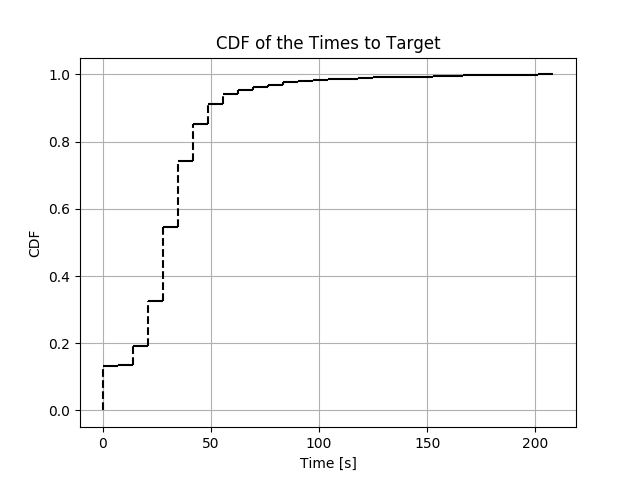
\includegraphics[width=0.5\textwidth]{../figures/cdf_total_time.png}
  \caption{The cumulative distribution of the participants' time taken to find a target object. }\label{fig:time-participants}
\end{figure}

In comparison to the VizWiz system~\cite{bigham2010vizwiz} (mean 92s, standard deviation 37.7s), our results look very reasonable. However, these results may greatly change when we test the system with participants with vision impairments.

\section{\uppercase{Conclusions}}\label{sec:conclusion}

\noindent In this work we presented and tested an MDP-based system to guide a person with vision impairments towards a target object with no apriori knowledge of the environment. We implemented the system in an Android app that we tested with a small group of sighted people to determine its viability and effectiveness at guiding a user to manipulating a camera and finding a target object. We found that is works well when compared to alternative systems, with a respectable mean time of target acquisition of 32s. However, the system can be improved by refining the search strategy and implementing an automatic fail-state recovery system that will guide a user back to neutral position if a fail-state is entered (e.g.\ a blank section of wall). Furthermore, a different dataset, purpose-built for object spatial relations, will give the MDP a more accurate understanding of the world and an improved transition model.

The next steps to this project will involve using the data recorded here to improve and refine the MDP model that provides the guidance. The model can also be expanded to include more objects and actions. However, an important consideration and expansion to the problem is to change the MDP to an Partially Observable MDP (POMDP) model that will bring the model more in line with reality by acknowledging that the objects are not perfectly observable and humans do not perfectly follow guidance instructions. This adjustment may be very important when we replace the QR code scanner with an object recognition that are typically more prone to making classification errors. Finally, the model can be adapted to use on-line learning techniques in order to further refine its transition model as the guidance system is used.  

% \clearpage
\bibliographystyle{apalike}
{\small
\bibliography{bib}}

\end{document}
